% =====================================================================
% Training dynamics: two figures per detector.
%   (a) four-variant comparison of the validation metrics
%   (b) loss components, baseline vs the recommended configuration
% Source: TrainingGrafs/*.png, per-epoch values from each run's results.csv.
% =====================================================================

\begin{figure*}[t]
\centering
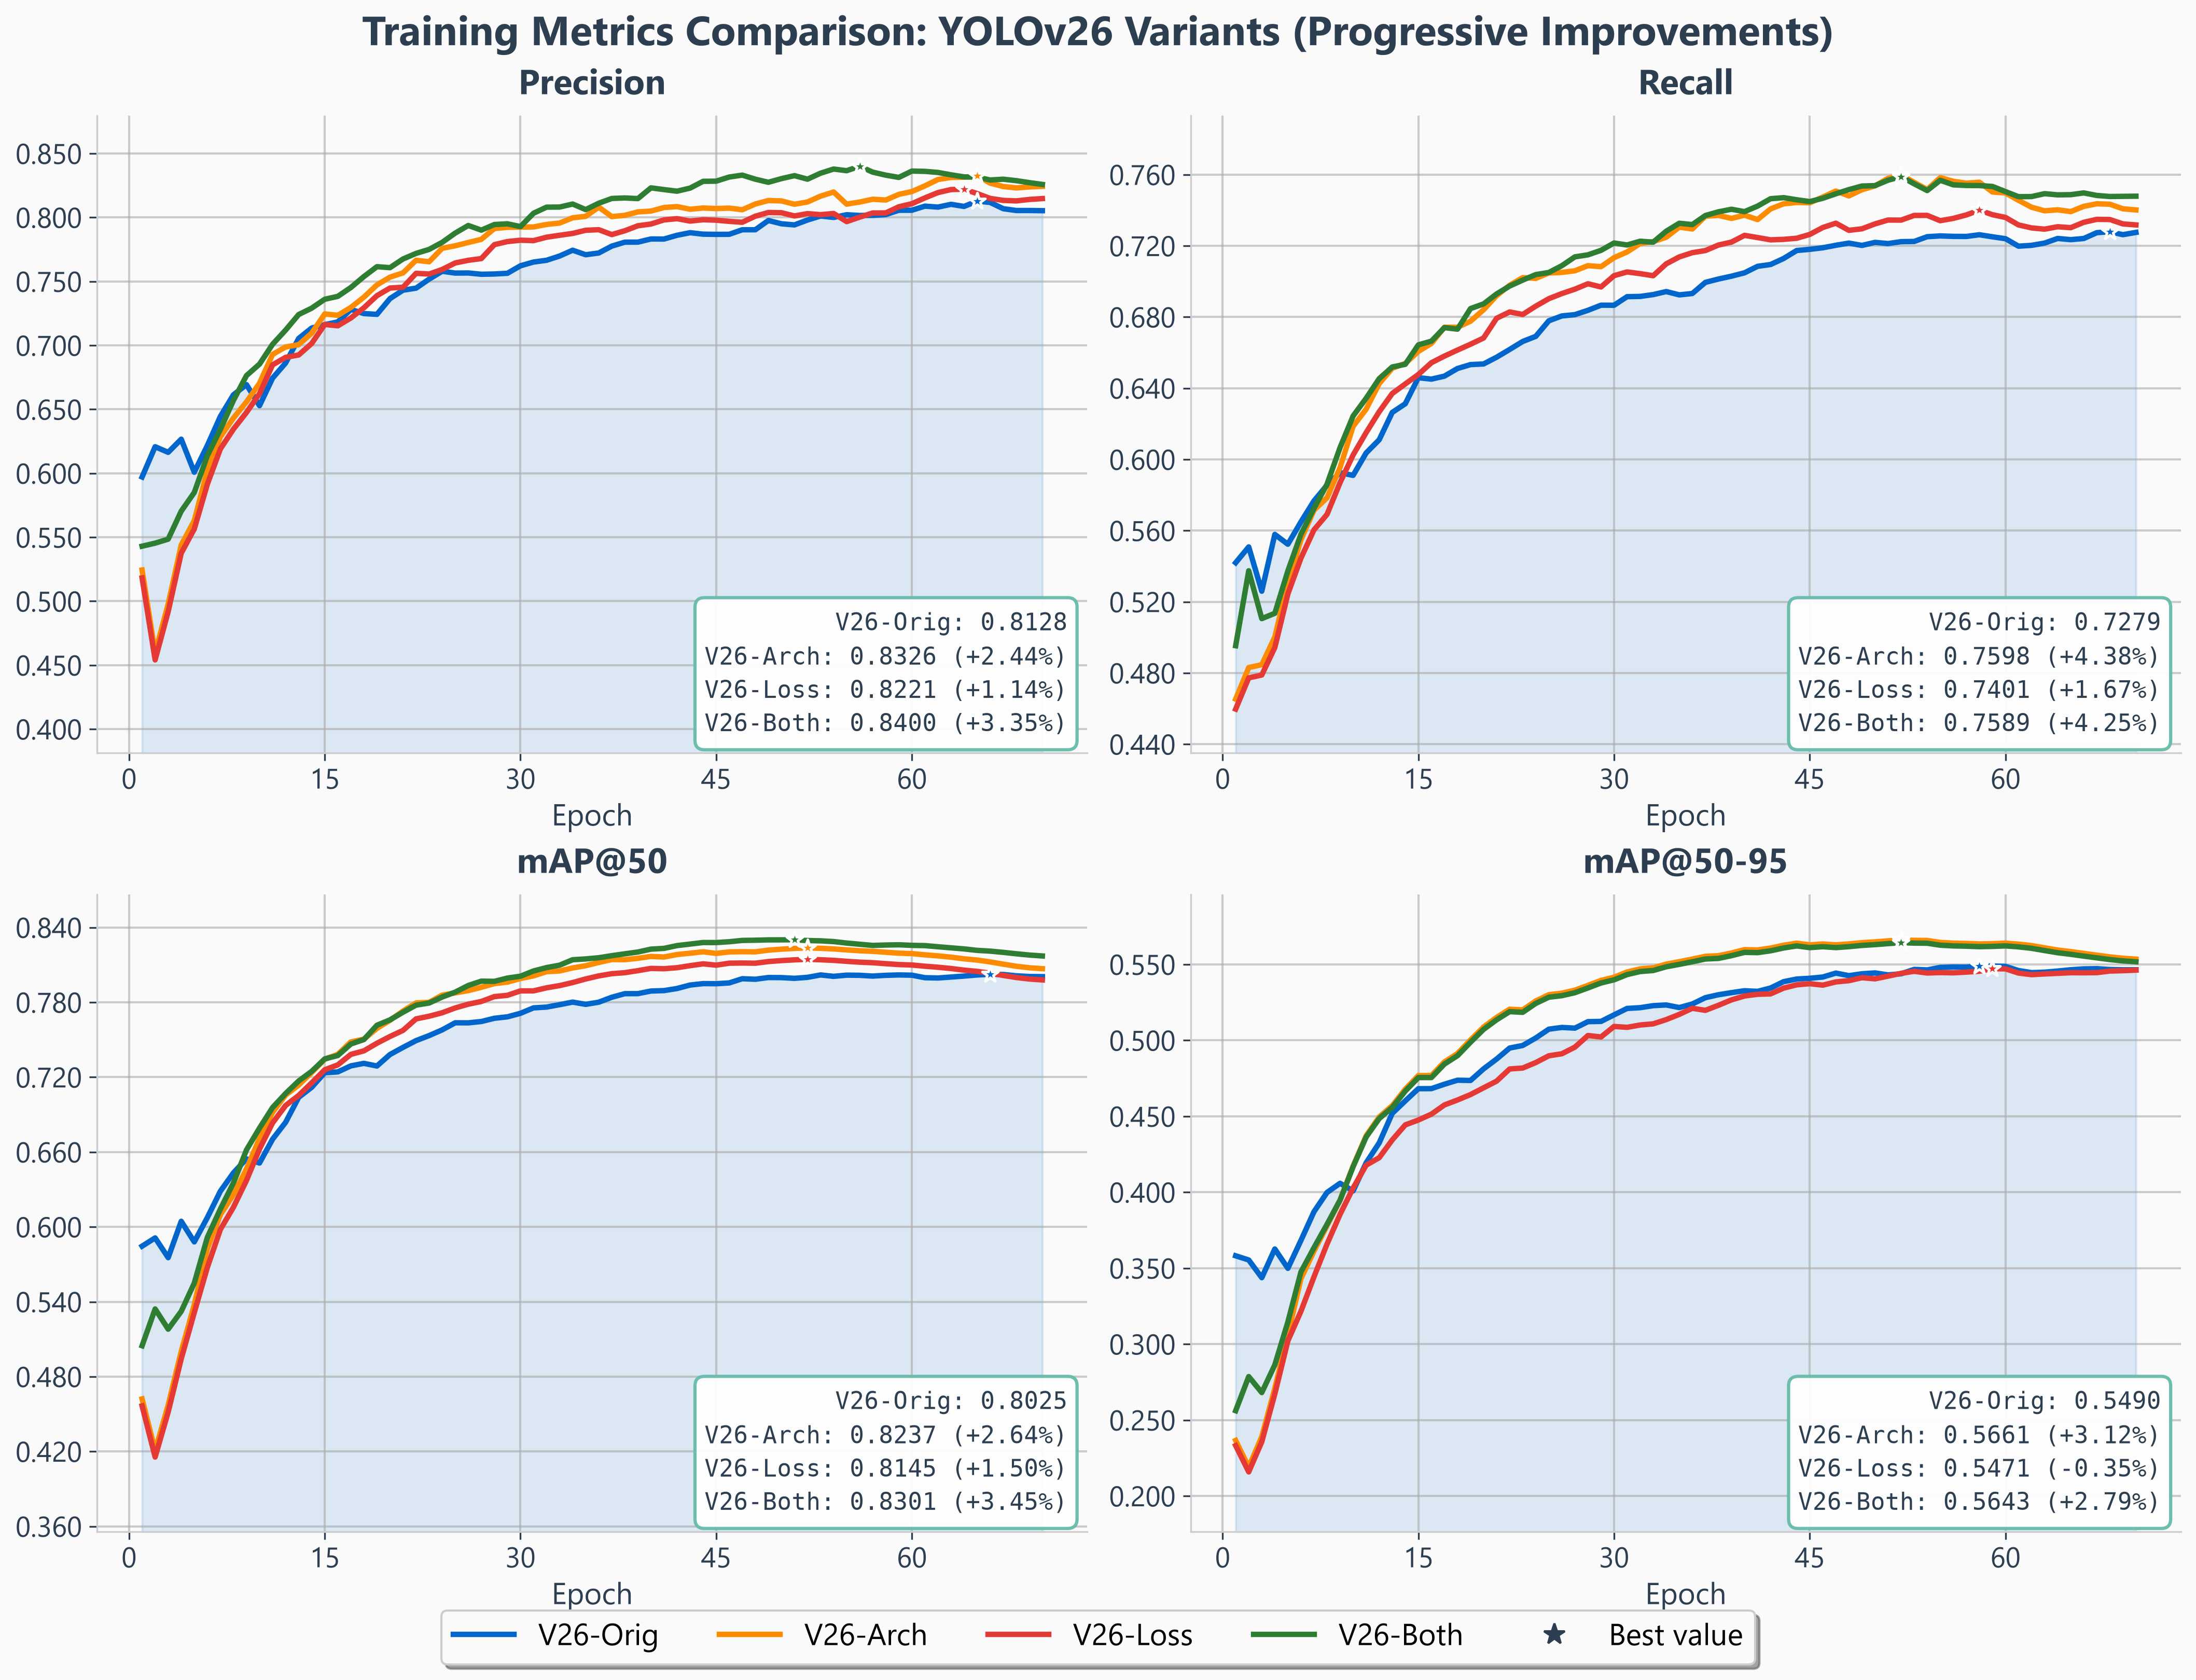
\includegraphics[width=0.98\linewidth]{TrainingGrafs/v26_metrics_4variant_compare.png}
\caption{YOLO26s training dynamics, all four configurations of
Table~\ref{tab:decomp}. Curves are per-epoch \textbf{validation} metrics; the
annotated end values are the corresponding \textbf{test} means over three seeds,
so they match Table~\ref{tab:decomp} rather than the curve maxima. The ordering
is established within the first fifteen epochs and never crosses, so the ranking
is not an artefact of where training stopped. Note the mAP$_{50\text{-}95}$
panel: the loss axis alone (red) tracks the baseline and ends slightly
\emph{below} it, which is the $-0.35\%$ of Table~\ref{tab:decomp} seen as a
trajectory.}
\label{fig:curves26}
\end{figure*}

\begin{figure*}[t]
\centering
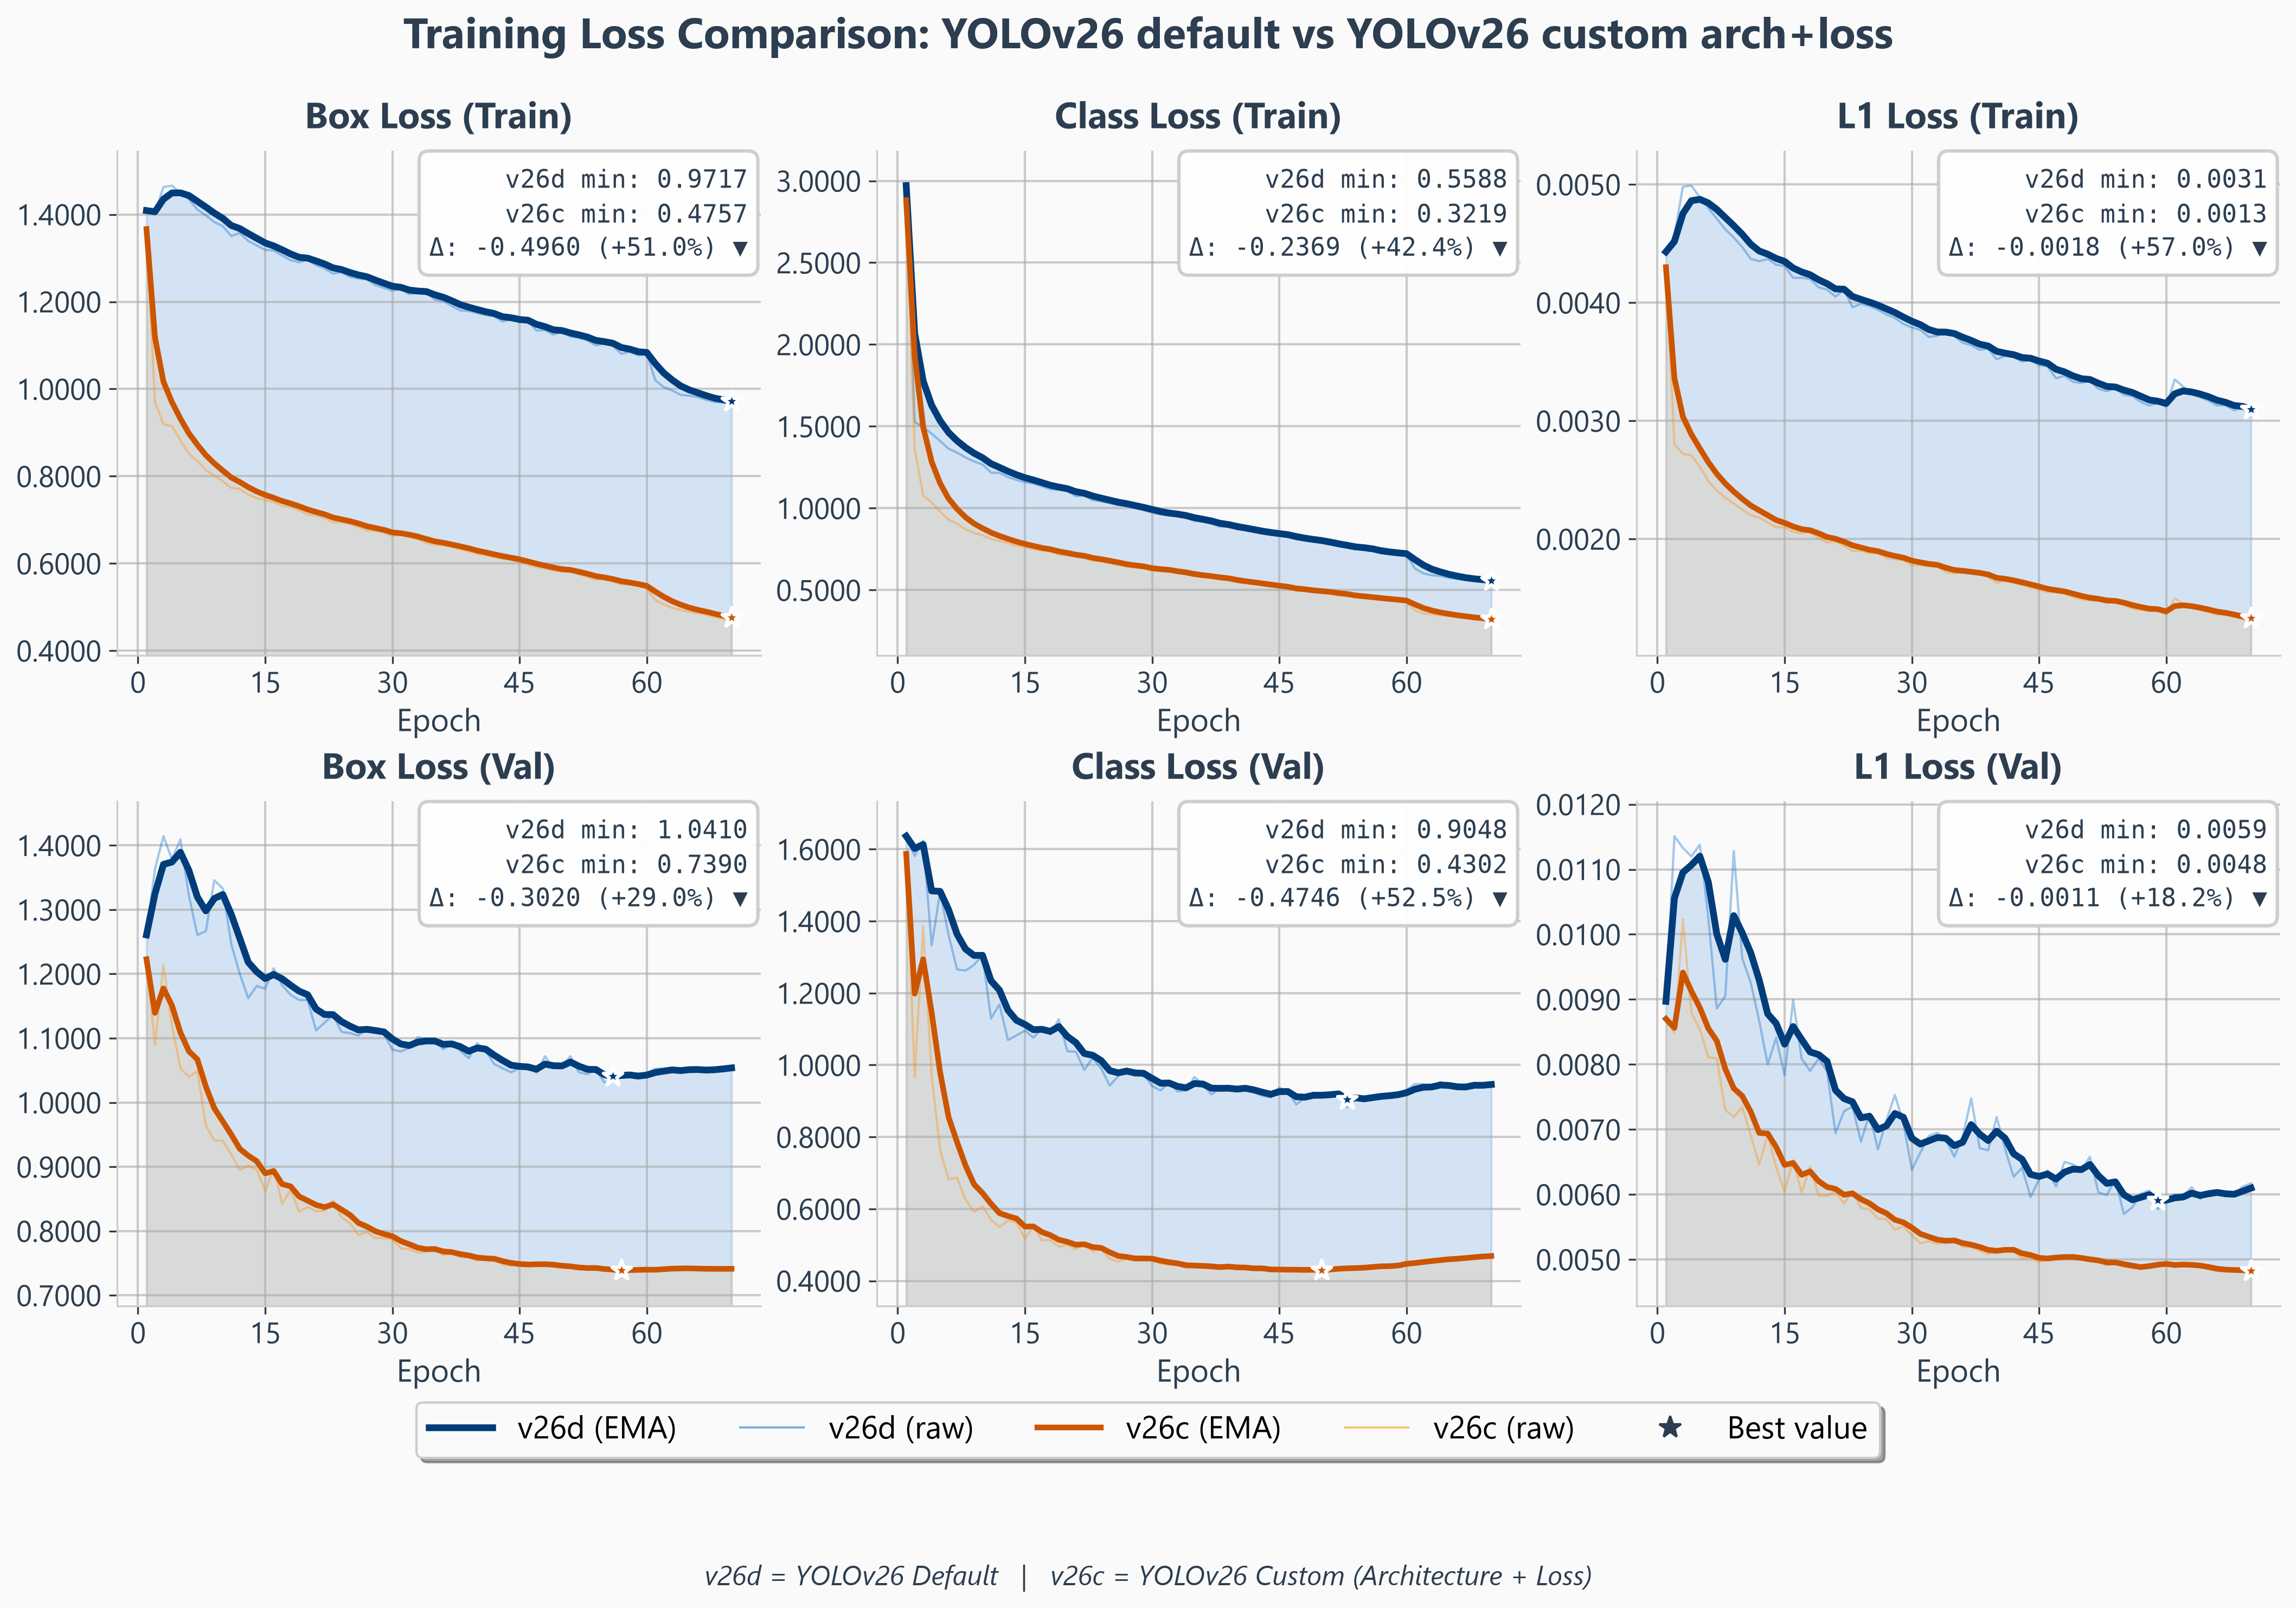
\includegraphics[width=0.98\linewidth]{TrainingGrafs/v26_metrics_loss_only.png}
\caption{YOLO26s \textbf{loss components}, baseline (\texttt{v26d}) versus the
recommended architecture$+$loss configuration (\texttt{v26c}); train on the top
row, validation on the bottom, EMA-smoothed in bold with the raw per-epoch
traces behind and the best value starred. Detection quality is not repeated
here --- the validation mAP, precision and recall curves are in
Fig.~\ref{fig:curves26}, where all four configurations can be compared at once.
All three terms fall substantially: box $-51.0\%$, classification $-42.4\%$ and
$\ell_1$ $-57.0\%$ on train, and $-29.0\%$, $-52.5\%$ and $-18.2\%$ on
validation, so the improvement is visible in the objective itself and not only
in the evaluated metrics. Both regression terms reach their validation minimum
late (box at epoch~$57$, $\ell_1$ at $60$) and stay flat to the end of the
schedule. The third panel is labelled \textbf{$\ell_1$ loss} rather than DFL:
YOLO26 sets $\mathrm{reg\_max}=1$ and substitutes an image-normalised $\ell_1$
term (Table~\ref{tab:implsdiff}), which is directly visible here and is the
structural difference Section~\ref{sec:disc:why} uses to explain why curriculum
area weighting does not transfer to this detector.}
\label{fig:loss26}
\end{figure*}

\begin{figure*}[t]
\centering

\includegraphics[width=0.98\linewidth]{TrainingGrafs/metrics_4variant_compare.png}
\caption{YOLOv12s training dynamics, same convention as
Fig.~\ref{fig:curves26}. The mAP$_{50\text{-}95}$ panel shows the same signature
as YOLO26 --- the loss axis alone ends $-0.37\%$ below the baseline while every
configuration containing the architecture ends above it --- which is the one
part of the loss mechanism's behaviour that is common to both detectors.}
\label{fig:curves12}
\end{figure*}

\begin{figure*}[t]
\centering
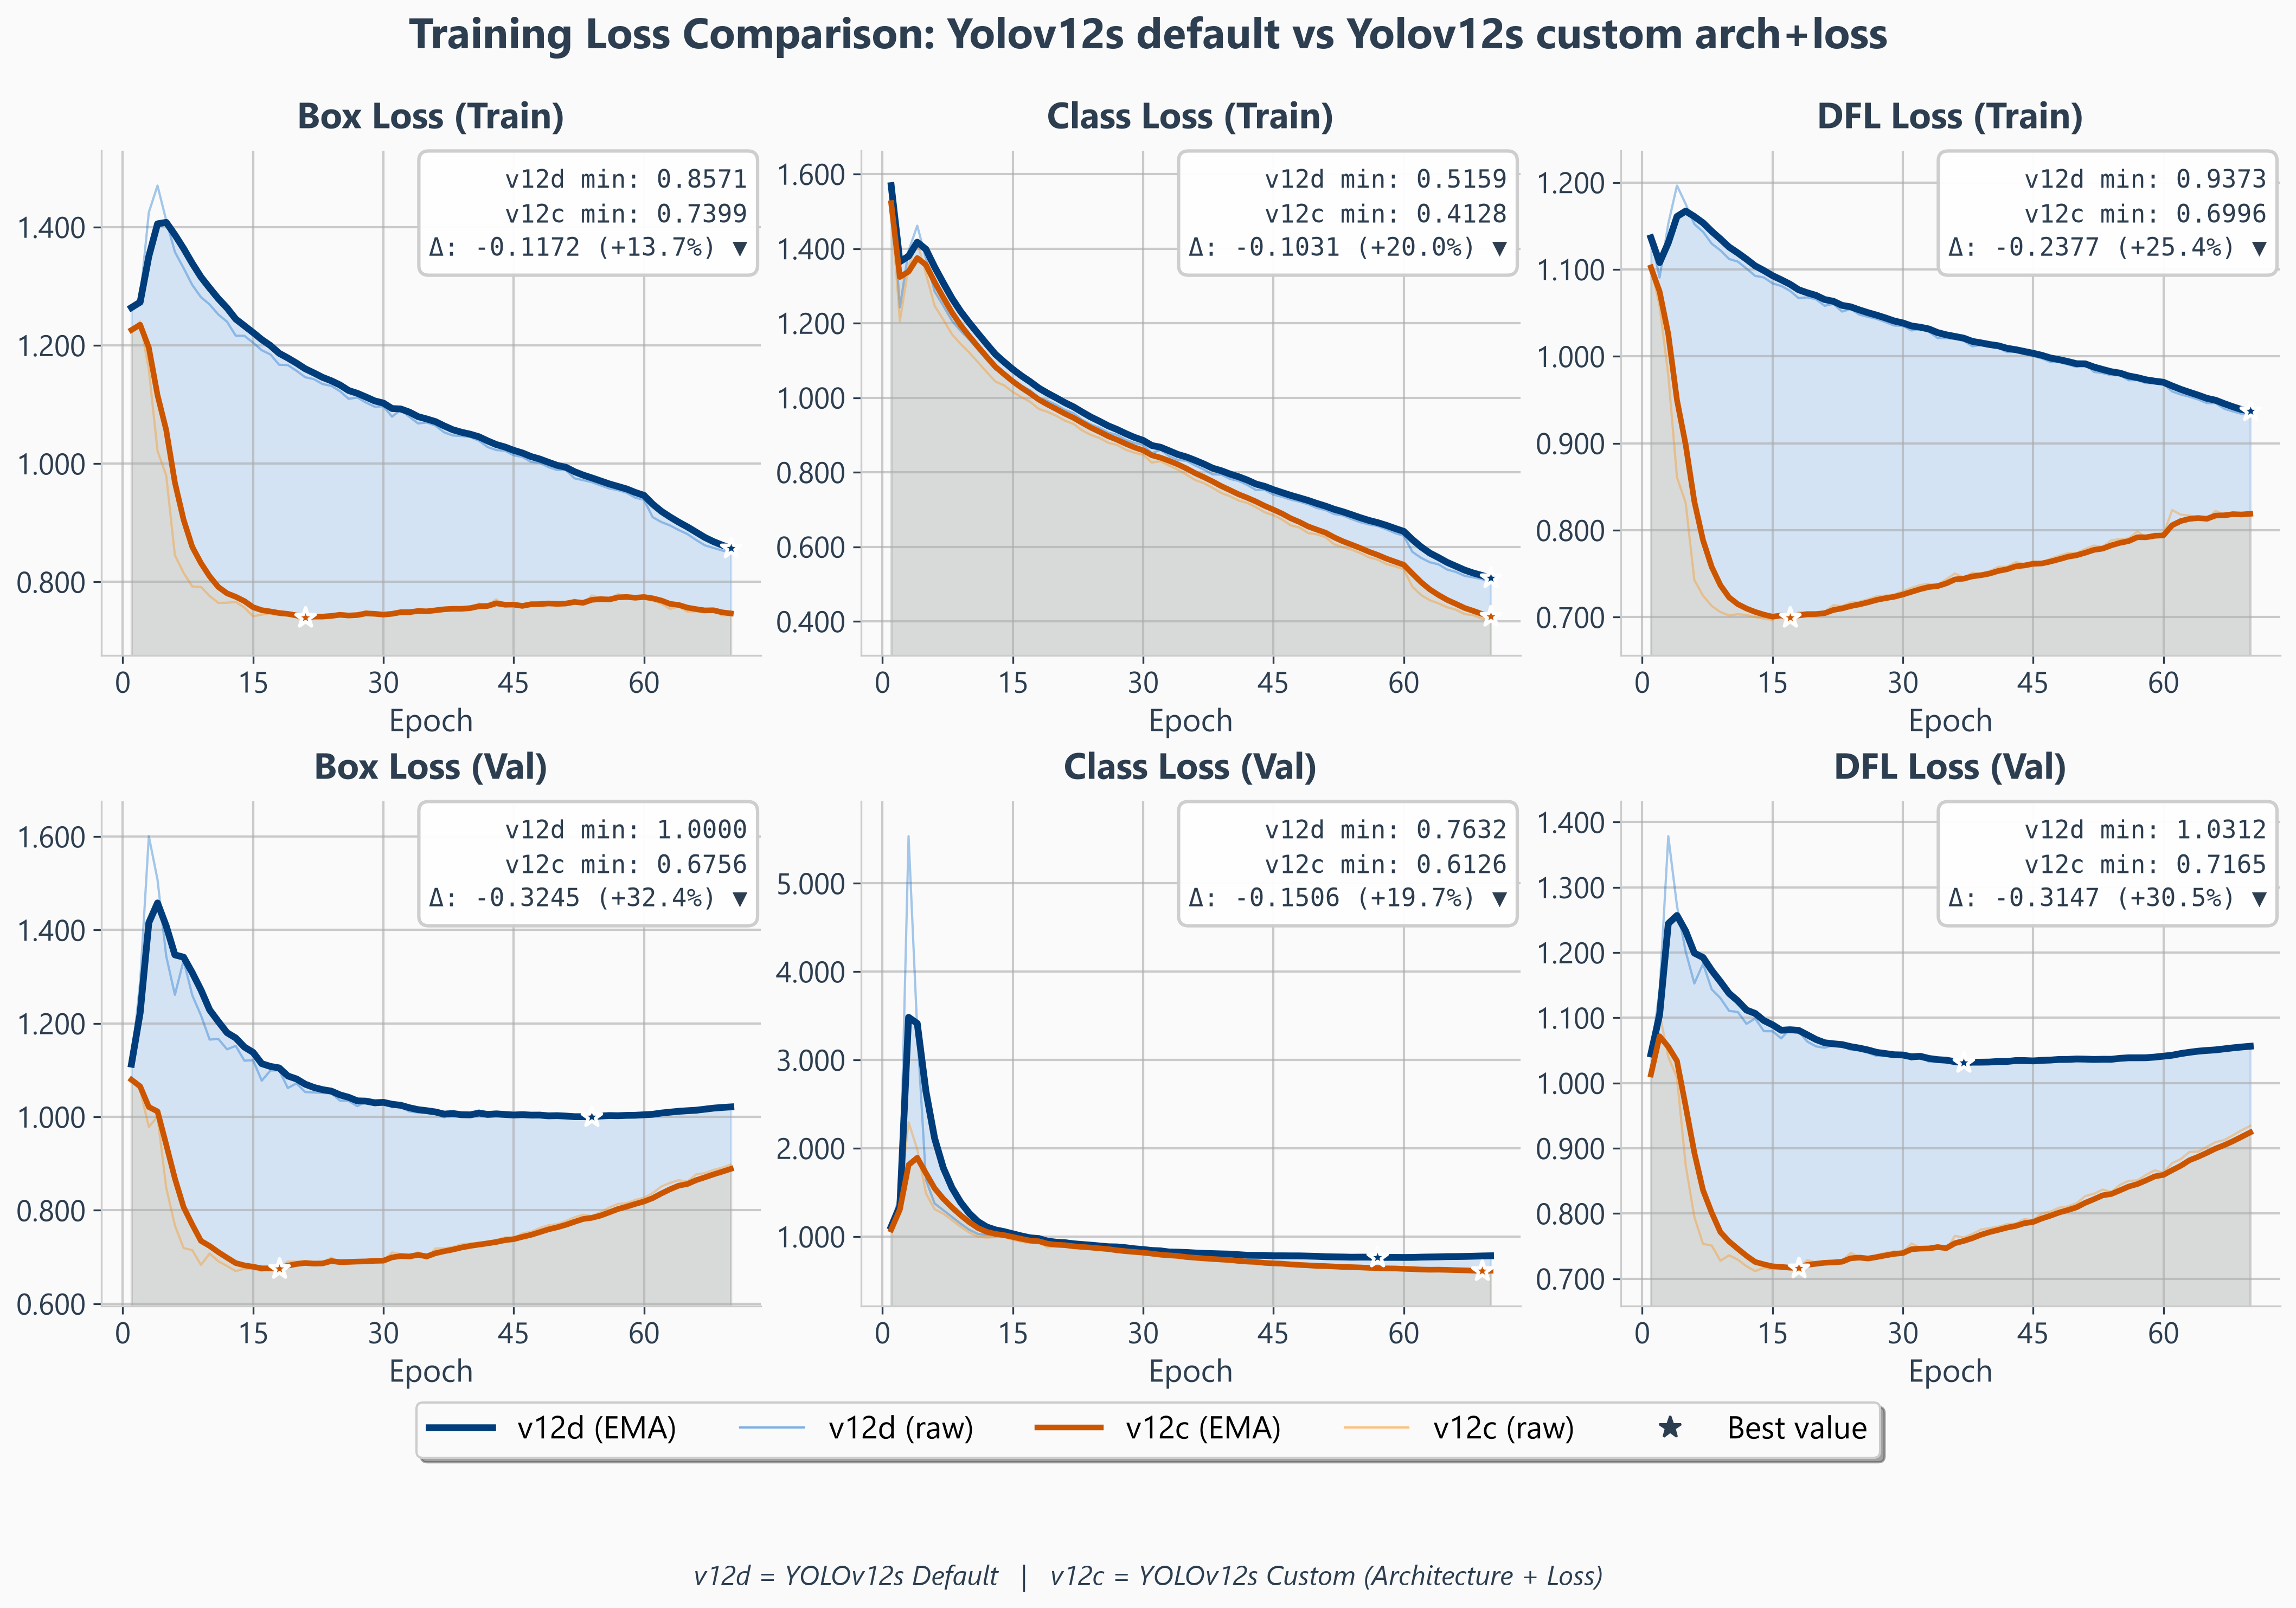
\includegraphics[width=0.98\linewidth]{TrainingGrafs/metrics_loss_only_v12.png}
\caption{YOLOv12s \textbf{loss components}, baseline (\texttt{v12d}) versus the
recommended configuration (\texttt{v12c}), same convention as
Fig.~\ref{fig:loss26}; the corresponding metric curves are in
Fig.~\ref{fig:curves12}. Box loss falls $13.7\%$ on train and $32.4\%$ on
validation, classification $20.0\%$ and $19.7\%$, DFL $25.4\%$ and $30.5\%$.
Two contrasts with Fig.~\ref{fig:loss26} matter. The third panel here is a
genuine \textbf{DFL} over $16$ bins, not an $\ell_1$ surrogate, which is the
difference Table~\ref{tab:implsdiff} records. And where YOLO26's regression
terms bottom out at the very end of the schedule, YOLOv12's reach their
validation minimum near epoch~$18$ --- box $0.676$, DFL $0.717$ --- and climb
steadily thereafter, while mAP$_{50}$ in Fig.~\ref{fig:curves12} keeps improving
to roughly epoch~$60$. The regression head overfits long before the detector
stops gaining, which is why checkpoints are selected on validation mAP rather
than on loss.}
\label{fig:loss12}
\end{figure*}
